% UTF-8 encoding
\documentclass[9pt, dvipsnames]{beamer} %

\usetheme[secheader]{Boadilla} 
\usecolortheme{default} 
\usefonttheme{professionalfonts} 
\usepackage{times}
\usepackage{amsmath}
\usepackage{verbatim}
\usepackage{listings}
\usepackage{anyfontsize}
\usepackage{subcaption} 
\usepackage{graphicx}
\usepackage[export]{adjustbox}
\setbeamertemplate{caption}[numbered]
\newcounter{saveenumi}
\resetcounteronoverlays{saveenumi}
\usepackage[multidot]{grffile}
\usepackage{tabularx}
\usepackage{tikz}
\usetikzlibrary{shapes, arrows}
\usepackage[utf8]{inputenc}
\usepackage[T1]{fontenc}

%%%%%%%%%%%%%%%%%%%

\pgfdeclareimage[width=8cm]{bgimage}{hub.png}

\usebackgroundtemplate{
\tikz\node[opacity=0.1,inner sep=0]{
	\vbox to \paperheight{\vfil\hbox to \paperwidth{\hfil
\includegraphics[width=8cm]{hub.png}\hfil}\vfil}
};
}


\setbeamercolor*{mycol}{bg=blue!89!black, fg=gray!10!white}

\makeatother
\setbeamertemplate{footline}
{
  \leavevmode%
  \hbox{%
  \begin{beamercolorbox}[wd=.3\paperwidth,ht=2.25ex,dp=1ex,center]{author in head/foot}%
    \usebeamerfont{author in head/foot}\insertshortauthor
  \end{beamercolorbox}%
  
  \begin{beamercolorbox}[wd=.42\paperwidth,ht=2.25ex,dp=1ex,center]{title in head/foot}
  	\usebeamerfont{title in head/foot}\insertshorttitle
  \end{beamercolorbox}
  \begin{beamercolorbox}[wd=.28\paperwidth,ht=2.25ex,dp=1ex,center]{date in head/foot}%
    \usebeamerfont{date in head/foot}
    \insertframenumber{} / \inserttotalframenumber\hspace*{1ex}
  \end{beamercolorbox}}%
  \vskip0pt%
}
\makeatletter

%%%%%%%%%%%%%%%%%%%
\setbeamertemplate{navigation symbols}{}


\title{The Bootstrap - Numerical Procedures and Applications} %
\author[Erin Sprünken]{Erin Sprünken\\
Humboldt-Universität zu Berlin} 
\date[11/2020]{20.11.2020}


\lstset{
   basicstyle=\ttfamily\small
}

\begin{document}

    \everymath{\displaystyle}

    % 标题页
    {\setbeamertemplate{footline}{} 
    \begin{frame}[noframenumbering]
        \titlepage 
    \end{frame}}
    \section*{Outline}
    \begin{frame}
        \frametitle{\textbf{Outline}}
        \tableofcontents
    \end{frame}
    \section{Motivation}
    \begin{frame}
    	\frametitle{\textbf{Motivation}}
    	An introductory example: Consider you are a researcher at Charité. Your colleagues and you are conducting research regarding a new treatment for lung cancer. In order to find out whether it is effective you need to undertake a trial with test subjects. However, for reasons you are not allowed to conduct a large-sample study. This reasons include the unknown (side-)effects as well as ethical reasons. Now, you have conflicting interests: On the one hand you want to have a large sample to get valid results and inference, on the other hand you are not allowed to. Your supervisor allows you to test the treatment among 10 test subjects. How can you get valid results?\\
 \hfill \\
    	Answer: Resampling Techniques
    	%\begin{itemize}
    %		\item Small Sample Sizes
    %		\item Asymptotic Results
    %		\item Tests
    %		\item Parameters
    %	\end{itemize}
    \end{frame}
    \section{Emphasis on Statistics and Finance}
    \begin{frame}
    	\frametitle{\textbf{General Applications}}
    	\begin{itemize}
    		\item Small sample sizes
    		\item Asymptotic results
    		\item Validation
    		\item Machine Learning techniques
    		\item Numerical solution to problems without analytical solution
    	\end{itemize}
    	\begin{alertblock}{ }
    		Other resampling techniques:
    		\begin{itemize}
    			\item Jackknife (precedes Bootstrap)
    			\item Cross-Validation (famous in Machine Learning)
    			\item Permutation (famous in two-sample problems)
    		\end{itemize}
    	\end{alertblock}
    \end{frame}
    \section{Theory}
    \begin{frame}
    	\frametitle{\textbf{Bootstrap Approach}}
    		\begin{block}{Pseudocode (General)}
    			\begin{enumerate}
    				\item Specify number of bootstrap iterations $nboot$
    				\item Fix Data $\mathbf{X} = (X_1, ..., X_n)$
    				\item For (i in 1:nboot)
    				\begin{enumerate}
    					\item Sample $\mathbf{X_i^{*}} = (X_{1}^{*}, ... X_{n}^{*})$ from $\mathbf{X}$
    					\item Compute Statistic of interest $\Psi(\mathbf{X_i^{*}})$
    					\item Save Statistic of interest at position $i$ in $\mathbf{\Psi} = (\Psi_1, ..., \Psi_i, ..., \Psi_{nboot})$
    				\end{enumerate}
					\item Use methods of statistical inference on the empirical distribution of $\mathbf{\Psi}$
    			\end{enumerate}
    		\end{block}
    \end{frame}
    \begin{frame}
    	\frametitle{\textbf{Why does that work?}}
    		We compute the bootstrap distribution. Since, given the fixed $\mathbf{X}$ the statistics of interest are random variables and we compute a sequence of random variables, we obtain an empirical distribution $\hat{F}_n$ of our variable of interest. Probability Theory taught us, that
    		\begin{align*}
    			\hat{F}_n(\psi) \quad \stackrel{\mathbb{P}-a.s.}{\to} \quad F(\psi).
    		\end{align*}
    		How do we bootstrap? My paper will focus on Nonparametric Bootstrap and (Rademacher-)Wild Bootstrap. 
	\end{frame}
	\begin{frame}
		\frametitle{\textbf{How does that work?}}
    		\begin{block}{Nonparametric Bootstrap}
    			\begin{itemize}
    				\item Fix Data $\mathbf{X} = (X_1, ..., X_n)$
    				\item In each iteration: Sample with replacement, such that $\mathbb{P}(X_1^{*} = X_1) = n^{-1}$
    				\item For valid asymptotic results this probability condition is necessary!
    				\item Each iteration consists of a bootstrap sample $\mathbf{X^{*}} = (X_1^{*}, ..., X_n^{*})$
    			\end{itemize}
    		\end{block}
    		\begin{block}{(Rademacher-) Wild Bootstrap}
    			\begin{itemize}
    				\item Fix Data $\mathbf{X} = (X_1, ..., X_n)$
    				\item Center Data $\mathbf{Z} = (Z_1, ..., Z_n)$ where $Z_k = X_k - \bar{X}$
    				\item In each iteration: Generate (sample) i.i.d. weights $\mathbf{w} = (w_1, ..., w_n)$ such that
    				\begin{align*}
    					\mathbb{E}[w_i] = 0, \quad Var(w_i) = 1 \qquad \forall i
    				\end{align*}
    				\item Generate Bootstrap sample $\mathbf{X^{*}} = (X_1^{*}, ..., X_n^{*})$, where $X_i^{*} = w_i \cdot Z_i$
    				\item Rademacher Distribution: $\mathbb{P}(w_i = 1) = \mathbb{P}(w_i = -1) = 0.5$
    			\end{itemize}
    		\end{block}
    \end{frame}
    \begin{frame}
    \frametitle{\textbf{One-sample t-Test}}
		\begin{block}{Problem}
			We want to test whether a population has a specific mean infering from a sample:
			\begin{align*}
				H_0: \qquad \mu \quad &= \quad \mu_0 \\
				H_1: \qquad \mu \quad &\neq \quad \mu_0
			\end{align*}			
			We infer from the sample mean.
		\end{block}		    	
    	\begin{alertblock}{Statistic}
    		\begin{align*}
    			T(\mathbf{X}) \quad &= \quad \frac{\bar{X} - \mathbb{E}[\bar{X}]}{Var(X)}\sqrt{n}
    		\end{align*}
    	\end{alertblock}
    \end{frame}
    
    \begin{frame}
    	\frametitle{\textbf{Bootstrapping the t-Test}}
    		\begin{block}{Pseudocode t-Test}
    			\begin{enumerate}
    				\item Specify number of bootstrap iterations $nboot$
    				\item Fix Data $\mathbf{X} = (X_1, ..., X_n)$
    				\item For (i in 1:nboot)
    				\begin{enumerate}
    					\item Sample$\mathbf{X^{*}} = (X_1^{*}, ..., X_n^{*})$ from $\mathbf{X}$
    					\item Compute Statistic $T_i(X^{*} \mid \mathbf{X})$
    				\end{enumerate}
    				\item Compute True Statistic $T(\mathbf{X})$
    				\item Decide whether to reject by comparing $T(\mathbf{X})$ to critical quantile of Bootstrap Distribution $\hat{T}_n$
    			\end{enumerate}
    		\end{block}
    \end{frame}
    \begin{frame}
    	\frametitle{\textbf{Bootstrapping the t-Test}}
    		\begin{alertblock}{Resampling Test Statistic}
				\begin{align*}
					T(X^{*} \mid \mathbf{X}) \quad &= \quad \frac{\bar{X}^{*} - \mathbb{E}[\bar{X}^{*} \mid \mathbf{X}]}{\hat{\sigma}^{*}} \sqrt{n} \\
					\bar{X}^{*} \quad &= \quad \frac{1}{n} \sum_{k=1}^n X_k^{*} \\
					(\hat{\sigma}^{*})^2 \quad &= \quad \frac{1}{n-1} \sum_{k=1}^n (X_k^{*} - \bar{X}^{*})^2 \\
					\mathbb{E}[\bar{X}^{*} \mid \mathbf{X}] \quad &= \quad \mathbb{E}\left[\frac{1}{n} \sum_{k=1}^n X_k^{*} \middle|\ \mathbf{X}\right] \\
					\mathbb{E}[X_k^{*} \mid \mathbf{X}] \quad &= \quad \bar{X}
				\end{align*}
    		\end{alertblock}
    \end{frame}
    \section{Computation}
    \begin{frame}
    	\frametitle{\textbf{Simulation and Computation}}
    	\begin{exampleblock}{What is of interest?}
    		\begin{itemize}
    			\item Accuracy
    			\item Speed and Complexity
    			\item Type I and (some) Type II Error
    		\end{itemize}
    	\end{exampleblock}
    	\begin{block}{Simulation Settings}
    		\begin{itemize}
    			\item Different distributions such as Normal, $\chi^2$, Exponential, ...
    			\item Different Datasets (Regression)
    			\item Different Implementations (R, C++ (with Rcpp), C) 
    			\item Different Number of Bootstrap Iterations
    			\item Different Bootstrap Versions (Nonparametric vs. Wild)
    		\end{itemize}
    	\end{block}
    	\begin{alertblock}{What is left out?}
    		\begin{itemize}
    			\item No Parametric Bootstrap
    			\item Only one version of Wild Bootstrap (Rademacher)
    			\item Regression Problem not available for Wild Bootstrap
    		\end{itemize}
    	\end{alertblock}
    \end{frame}
    \begin{frame}
    	\frametitle{\textbf{What is of interest?}}
    	\begin{block}{Accuracy}
    		\begin{align*}
    			Bias \quad &= \quad \mathbb{E}[\hat{\theta} - \theta]\\
    			Variance \quad &= \quad \mathbb{E}\left[(\hat{\theta} - \mathbb{E}[\theta])^2\right] \\
    			\Rightarrow MSE \quad &= \quad Variance + Bias^2
    		\end{align*}
    	\end{block}
    	\begin{block}{Speed and Complexity}
    		\begin{itemize}
    			\item Complexity is qualitative: How hard is it to write or read the code
    			\item Speed is quantitative: How long do the computations take
    		\end{itemize}
    	\end{block}
    	\begin{block}{Type I and Type II Error}
    		\begin{align*}
    			\alpha \quad &= \quad \mathbb{P}(H_1 \mid H_0) \\
    			1 - \beta \quad &= \quad \mathbb{P}(H_0 \mid H_1)
    		\end{align*}
    	\end{block}
    \end{frame}
    \begin{frame}
    	\frametitle{\textbf{Computational Issues and Implementation}}
    		Best Practice and it's importance in R:\\
    		R is a very handy language regarding statistics. Why should we even stick to best practices such as matrix algebra, if the code works it works, right?
    		\begin{alertblock}{Wrong!}
    			R is a very-high-level language. What does that mean? From low to high we have:
    			\begin{enumerate}
    				\item Machine Code
    				\item Assembler
    				\item C, FORTRAN
    				\item R, Python, ...
    			\end{enumerate}
    			Implementations in R which do not follow Best Practice can lead to very inefficient programs which can cost a huge amount of time. This is, because the computer has to go all the steps from R to machine Code. See the following examples for a simple bootstrap version of the one-sample t-Test.
    		\end{alertblock}
    \end{frame}
    \begin{frame}[fragile]
    	\frametitle{\textbf{Example: Not Best Practice R}}
    	Why is this not best practice? We make use of for loops and ignore the matrix-structure of R
    	\begin{block}{Code main part of t-Test}
    	\begin{verbatim}
T.x    = c()
t.true = (mean(x) - mu.0) / sqrt(var(x)) * sqrt(length(x))

for(i in 1:nboot){
    x.boot = sample(x, size = length(x), replace = T)
    t.boot = (mean(x.boot) - mean(x)) /
              sqrt(var(x.boot))*sqrt(length(x))
    T.x = c(T.x, t.boot)
}
    	\end{verbatim}
    	\end{block}
    \end{frame}
    \begin{frame}[fragile]
    	\frametitle{\textbf{Example: Best Practice R}}
    	In this example we exploit the matrix-structure of R resulting in a far more efficient computation. Some of you may know the usage of the apply-family to avoid for-loops, but matrix-algebra will usually be superior to apply in terms of efficency. The reason is, that apply is yet another for-loop in R. Matrix-functions in R are computed in C and thus highly competetive when it comes to speed.
		\begin{block}{Code main part of t-Test - Best Practice}
    	\begin{verbatim}
T.x    = numeric(nboot)
n      = length(x)
t.true = (mean(x) - mu.0) / sqrt(var(x)) * sqrt(n)
x.boot = matrix(sample(x, size = n*nboot, replace = T),
         ncol = nboot)
x.mean = colMeans(x.boot)
x.var  = (colSums(x.boot^2) - n*x.mean^2)/(n-1)
T.x    = sqrt(n) * (x.mean - mean(x)) / sqrt(x.var)
    	\end{verbatim}
		\end{block}
    \end{frame}
   	\begin{frame}
    	\frametitle{\textbf{Results: Best Practice vs. Not Best Practice}}
    	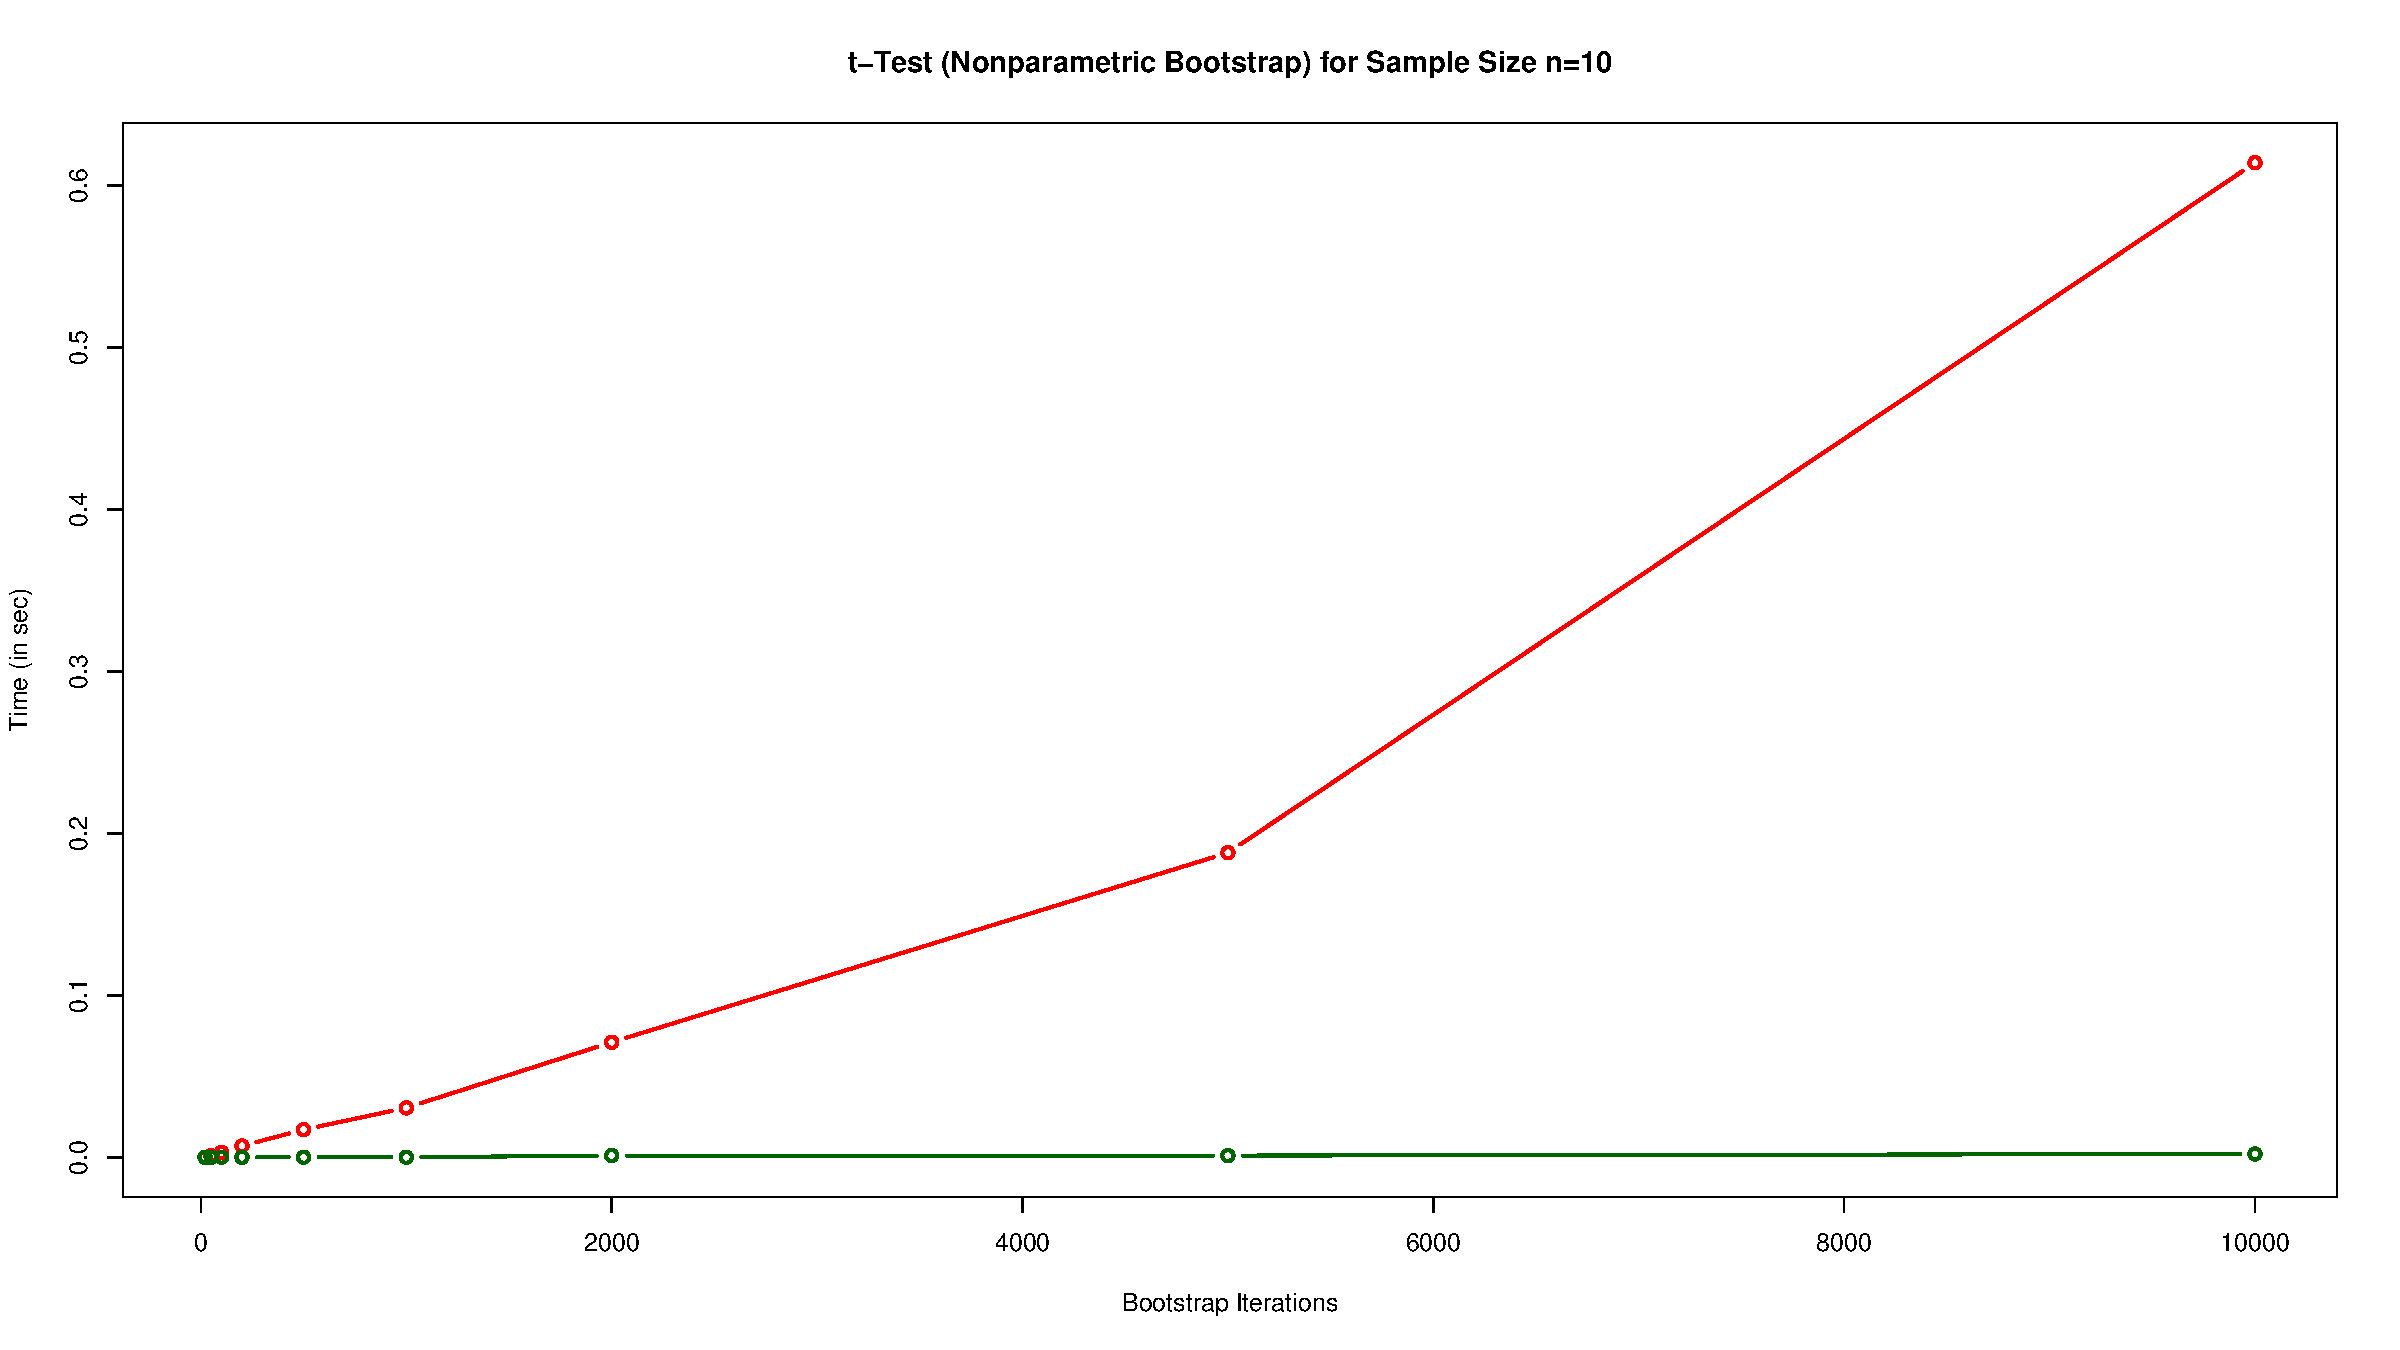
\includegraphics[scale=0.3]{time1}
    	Red Line: Loop-Version, Green Line: Matrix-Version
   	\end{frame}
   	\section{Outlook}
	\begin{frame}
		\frametitle{\textbf{What can be done beyond my seminar paper?}}
		\begin{itemize}
			\item Multiple Contrast Tests
			\item Effect-Size Tests
			\item Multivariate-Behrens-Fisher Problem
			\item Other Tests (Anderson-Darling, Shapiro-Wilk, ...)
			\item Timeseries Bootstrapping
			\item Bootstrapping in Portfolio Analysis
			
		\end{itemize}
	\end{frame}
	\begin{frame}
		\frametitle{Literature}
			\begin{itemize}
				\item Bootstrap Methods: Another Look at the Jackknife (Efron, 1979)
				\item Estimated Sampling Distributions: The Bootstrap and Competitors (Beran, 1982)
				\item Jackknife, Bootstrap and Other Resampling Methods in Regression Analysis (Wu, 1986)
				\item Bootstrap, wild bootstrap and asymptotic normality (Mammen, 1992)
				\item Bootstrapping and permuting paired t-test type statistics (Konietschke and Pauly, 2014)
			\end{itemize}
	\end{frame}
\end{document}